\documentclass[crop, tikz]{standalone}

\usetikzlibrary{math}
\usetikzlibrary{calc}
\usetikzlibrary{positioning}
\begin{document}
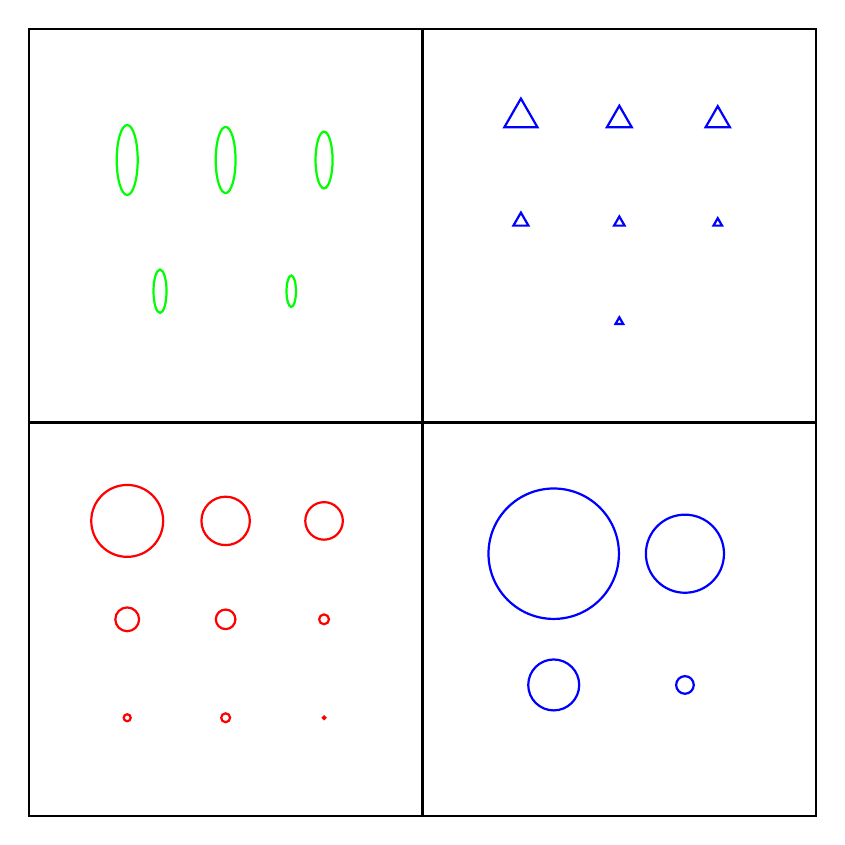
\begin{tikzpicture}
  \draw[thick] (0, 0) rectangle (5, 5);
  \draw[thick] (5, 0) rectangle (10, 5);
  \draw[thick] (0, 5) rectangle (5, 10);
  \draw[thick] (5, 5) rectangle (10, 10);

  % red circles
  % import numpy as np
  % for x, y, r in zip(10*(np.random.random(5)), 10*(np.random.random(5)), 0.5*(np.random.random(5))):
  %     print(str(x)+'/'+str(y)+'/'+str(r)+',')

  \foreach \xcord / \ycord / \rcord in {
    {1*5/4} / {3*5/4} / 0.4565838404947177,
    {2*5/4} / {3*5/4} / 0.3074134849629631,
    {3*5/4} / {3*5/4} / 0.23838775192054612,
    {1*5/4} / {2*5/4} / 0.15078170372073274,
    {2*5/4} / {2*5/4} / 0.12417262955376379,
    {3*5/4} / {2*5/4} / 0.06244327990940718,
    {1*5/4} / {1*5/4} / 0.044592439438311426,
    {2*5/4} / {1*5/4} / 0.05653784106297699,
    {3*5/4} / {1*5/4} / 0.014712651759808348
  }{
    \draw[red, thick] (\xcord, \ycord) circle (\rcord);
  }

  % blue circles
  \foreach \x / \y / \r in {
    {5+1*5/3} / {2*5/3} / 0.8282351326975819,
    {5+2*5/3} / {2*5/3} / 0.4959151367782896,
    {5+1*5/3} / {1*5/3} / 0.32343724210759717,
    {5+2*5/3} / {1*5/3} / 0.11194328613448434
  }{
    \draw[blue, thick] (\x,\y) circle (\r);
  }

  % green ellipses
  \foreach \x / \y / \a / \b in {
    {1*5/4} / {5+2*5/3} / 0.44458636535075624 / 0.13337590960522686  ,
    {2*5/4} / {5+2*5/3} / 0.42017352508362876 / 0.12605205752508863  ,
    {3*5/4} / {5+2*5/3} / 0.36019401697947695 / 0.10805820509384308  ,
    {1*5/3} / {5+1*5/3} / 0.27526797473586584 / 0.08258039242075975  ,
    {2*5/3} / {5+1*5/3} / 0.19991550807517933 / 0.059974652422553794
  }{
    \draw[green, thick] (\x, \y) ellipse (\b cm and  \a cm);
  }

  % blue triangles
  % import numpy as np
  % for x, y, a, ang in zip(10*(np.random.random(5)), 10*(np.random.random(5)), 0.5*(np.random.random(5)), 180*(np.random.random(5))):
  %    print(str(x)+'/'+str(y)+'/'+str(a)+'/'+str(0.3*a)+'/'+str(ang)+',')

  % This computation of the x coords is ugly as all hell. Need to right
  % shift the triangles by \a/2 since they're anchored at the bottom right
  % corner. Couldn't get it to work in the foreach loop.
  \foreach \x / \y / \a in {
    {5+1*5/4+0.419809206167695/2}   / {5+3*5/4} / 0.419809206167695  ,
    {5+2*5/4+0.31485139062877743/2} / {5+3*5/4} / 0.31485139062877743,
    {5+3*5/4+0.3076868629010771/2}  / {5+3*5/4} / 0.3076868629010771 ,
    {5+1*5/4+0.19102094661889218/2} / {5+2*5/4} / 0.19102094661889218,
    {5+2*5/4+0.13385616813162254/2} / {5+2*5/4} / 0.13385616813162254,
    {5+3*5/4+0.10883725448703785/2} / {5+2*5/4} / 0.10883725448703785,
    {5+2*5/4+0.09875441625998671/2} / {5+1*5/4} / 0.09875441625998671
  }{
    \draw[blue, thick] (\x,\y) \foreach \s in {120, 240}{
      -- ++ (\s:\a)
    } -- cycle ++ (90:\a);
  }
\end{tikzpicture}
\end{document}
